\documentclass[11pt]{report}

% Paquetes y configuraciones adicionales
\usepackage{graphicx}
\usepackage[export]{adjustbox}
\usepackage{caption}
\usepackage{float}
\usepackage{titlesec}
\usepackage{geometry}
\usepackage[hidelinks]{hyperref}
\usepackage{parskip}
\usepackage{hyperref}
\usepackage{nameref}
\usepackage{fontspec}
\usepackage{listings}
\usepackage{wrapfig}

% Configura la fuente
% \setmainfont{Geist}


% Configura los márgenes
\geometry{
    left=2cm,   % Ajusta este valor al margen izquierdo deseado
    right=2cm,  % Ajusta este valor al margen derecho deseado
    top=2cm,
    bottom=2cm,
}

% Redefinir el formato del capítulo
\titleformat{\chapter}[block]
  {\normalfont\huge\bfseries}{\chaptertitlename\ \thechapter}{1em}{\Huge}

% Ajustar el espaciado antes y después del título del capítulo
\titlespacing*{\chapter}{0pt}{0pt}{20pt}

% Configuración de los títulos de las secciones
\titlespacing{\section}{0pt}{\parskip}{\parskip}
\titlespacing{\subsection}{0pt}{\parskip}{\parskip}
\titlespacing{\subsubsection}{0pt}{\parskip}{\parskip}


\begin{document}

% Portada del informe

\title{Linked Data}
\author{Samuel Martín Morales  \texttt{alu0101359526@ull.edu.es} \and Jorge Domínguez González  \texttt{alu0101330600@ull.edu.es} \and Juan Diego Rendon Cachafeiro \texttt{alu0101327747@ull.edu.es}}
\date{\today}

\maketitle

% Índice
\tableofcontents

% Secciones del informe
\chapter{Introducción}

En la última década, la web ha experimentado una transformación fundamental desde una simple red de información hacia lo que hoy se conoce como \textbf{Linked Data} o \textbf{datos enlazados}. Este cambio, impulsado por la evolución de la web semántica, ha llevado a la adopción de un paradigma que va más allá de la  presentación de información en forma de texto. Linked Data propone una visión donde los datos adquieren una estructura que facilita la creación de conexiones y enlaces entre diversos conjuntos de datos, provenientes incluso de fuentes y proveedores distintos.

De manera general, Linked Data representa un conjunto de prácticas sólidas para la publicación y conexión de datos estructurados en la web. Haciendo uso de tecnologías del W3C, como \textbf{URIs}, el \textbf{protocolo HTTP} y el modelo de datos \textbf{RDF} o \texttt{\textbf{Resource Description Framework}}, se establece una base que permite la identificación única de entidades, la recuperación de recursos y la descripción detallada de los mismos.

En el presente informe se tiene como objetivo explorar los fundamentos de Linked Data, desde sus principios esenciales hasta su aplicación práctica. En esencia este se centrará en cómo las URIs, el protocolo HTTP y el modelo RDF forman parte de la revolución semántica, permitiendo la interconexión de datos. Además, se examinará el impacto del Linked Open Data (LOD) y cómo este enfoque híbrido entre \texttt{datos enlazados} y \texttt{datos abiertos} está transformando la forma en la que se accede, se utiliza y se comparte la información en un mundo cada vez más interconectado.

\chapter{Linked Data}

\section{Componentes de Linked Data}

Para comenzar con el estudio de Linked Data, es necesario entender los componentes que lo conforman. En este sentido, se puede decir que Linked Data se basa en tres pilares fundamentales: URIs, HTTP y RDF. A continuación, se describirá cada uno de estos componentes y se explicará su importancia en el contexto de Linked Data.

- URI (Identificadores de recursos uniformes): Una URI es una cadena de caracteres que identifica de manera única un recurso en la web. En este perspectiva, se puede decir que una URI es un identificador de recursos uniforme, ya que, permite la identificación de los distintos recursos en la web de una manera uniforme y consistente. Además, las URIs son utilizadas por los agentes de software para acceder a los recursos de esta. \ref{subsec:Uniformidad-URIs}

- HTTP (Protocolo de Transferencia de Hipertexto): Se hace uso del protocolo HTTP para que las URIs sean desreferenciables. Esto quiere decir que, al acceder a una URI mediante el protocolo HTTP se debe de obtener información sobre el recurso al que hace referencia la URI. Además, el protocolo HTTP permite la recuperación de recursos a través de la web. En este sentido, se puede decir que el protocolo HTTP es el protocolo de la web, ya que, es el protocolo que permite la recuperación de recursos a través de esta. \ref{subsec:Características-HTTP}

- RDF (Marco de Descripción de Recursos): RDF es un modelo estándar para describir recursos y sus relaciones haciendo uso de tripletes (sujeto, predicado, objeto). \ref{subsec:Características-RDF}

- Enlaces entre recursos: Las URIs deben de incluir enlaces (enlaces de hipertexto) a otras URIs, de esta manera se pueden establecer relaciones entre los recursos y la navegación entre estos. Esto lo que permite es la fomentación de la creación de una red interconectada de datos en la web.

Estos componentes permiten que los datos estén interconectados, facilitando por un lado la navegación y el descubrimiento de información relacionada. Por tanto, cuando se siguen estos principios, se puede decir que los datos están enlazados (\textbf{Linked Data}), siendo estos datos fundamentales para la construcción de la web semántica, dónde, la información tiene un significado definido y las máquinas pueden entender y procesar los datos de manera efectiva.

\subsection{Uniformidad de las URIs} \label{subsec:Uniformidad-URIs}

\indent \indent \indent -  \textbf{Unicidad}: Cada recurso debe tener una URI única. La unicidad garantiza que no haya conflictos ni duplicados en la identificación de los recursos. Cada URI debería de ser única en el ámbito global de la web.

\indent \indent \indent -  \textbf{Consistencia}: Las URIS deben de seguir un formato consistente y estandarizado. Esto permite la facilidad de comprensión y manejo por parte tanto de las máquinas como de las personas. Además, permite el establecimiento de patrones y la simplificación de su uso.

\indent \indent \indent -  \textbf{Persistencia}: Las URIs deben de ser persistentes. Esto quiere decir que una URI debe de ser válida y accesible en todo momento. De esta manera, se garantiza que los recursos puedan ser accedidos en el momento que se considere.

\indent \indent \indent -  \textbf{Desreferenciables}: Las URIs deben de ser desreferenciables. Es decir, el acceder a una URI mediante el protocolo \texttt{HTTP} se debe de obtener información sobre el recurso al que hace referencia la URI. Esto permite que las URIs no solo se traten de identificadores únicos, sino 	que también sean enlaces a información relevante.

\subsection{Características del protocolo HTTP} \label{subsec:Características-HTTP}

\indent \indent \indent - \textbf{Cliente-Servidor}: El protocolo HTTP se basa en un modelo cliente-servidor. Esto quiere decir que, el cliente realiza una petición al servidor y este le responde con la información solicitada. En este sentido, el cliente es el agente de software que realiza la petición y el servidor es el agente de software que responde a la petición.

\indent \indent \indent - \textbf{Sin estado}: El protocolo HTTP es un protocolo sin estado. Es decir, cada petición que se realiza al servidor es independiente de las demás. Por tanto, el servidor no guarda información sobre las peticiones anteriores. Esto permite que el protocolo sea simple y fácil de implementar.

\indent \indent \indent - \textbf{Protocolo de aplicación}: Se trata de un protocolo de nivel de aplicación utilizado para la transferencia de información en la WWW (\texttt{World Wide Web}). De manera general, opera en la capa de aplicación del modelo OSI (\texttt{Open Systems Interconnection}) \cite{1}.

\indent \indent \indent - \textbf{Mensajes}: Las comunicaciones se realizan mediante mensajes. Un solicitud de un cliente y una respuesta del servidor consisten en un encabezado y de manera opcional en un cuerpo. El encabezado contiene la información sobre dicha solicitud o respuesta y el cuerpo contiene la información que se quiere transmitir.

\indent \indent \indent - \textbf{URis}: Las distintas solicitudes y respuestas en HTTP hacen uso de identificadores de recursos uniformes para identificar los distintos recursos en la web. Esto lo que permite, es especificar la ubicación y el nombre del recurso.

\indent \indent \indent - \textbf{Basado en texto}: Las distintas solicitudes y respuestas se codifican en texto.  Esto lo que permite es que se facilita la comprensión y el procesamiento de las solicitudes y respuestas tanto por parte de los humanos como de las propias máquinas.

\indent \indent \indent - \textbf{Métodos}: El protocolo define una serie de métodos que se utilizan para poder indicar la acción que el cliente quiere realizar. Algunos de los métodos más comunes son GET, POST, PUT, DELETE, etc.

\subsection{Características de RDF} \label{subsec:Características-RDF}

\indent \indent \indent - \textbf{Reutilización}: RDF hace uso de URIs para identificar los recursos, permitiendo la facilidad en la reutilización de la información RDF en diferentes aplicaciones.

\indent \indent \indent - \textbf{Interoperatividad}: Este está estandarizado por el W3C \cite{5}, lo que permite que diferentes aplicaciones RDF puedan trabajar juntas más fácilmente.

\indent \indent \indent - \textbf{Extensibilidad}: RDF permite la extensión de vocabularios RDF existentes, lo que permite la creación de vocabularios RDF más específicos.

\indent \indent \indent - \textbf{Escalabilidad}: Se puede hacer más grande según sea necesario (escalable),  permitiendo que se pueda usar para representar grandes cantidades de información o datos.

\section{Esquematización de los componentes de Linked Data}

Teniendo en cuenta todo esto anterior, se puede observar a continuación una esquema de todo lo comentado anteriormente, de tal manera que los conceptos básicos puedan ser comprendidos de manera más sencilla \ref{fig:Componentes-Linked-Data}.

\begin{figure}[H]
	\centering
	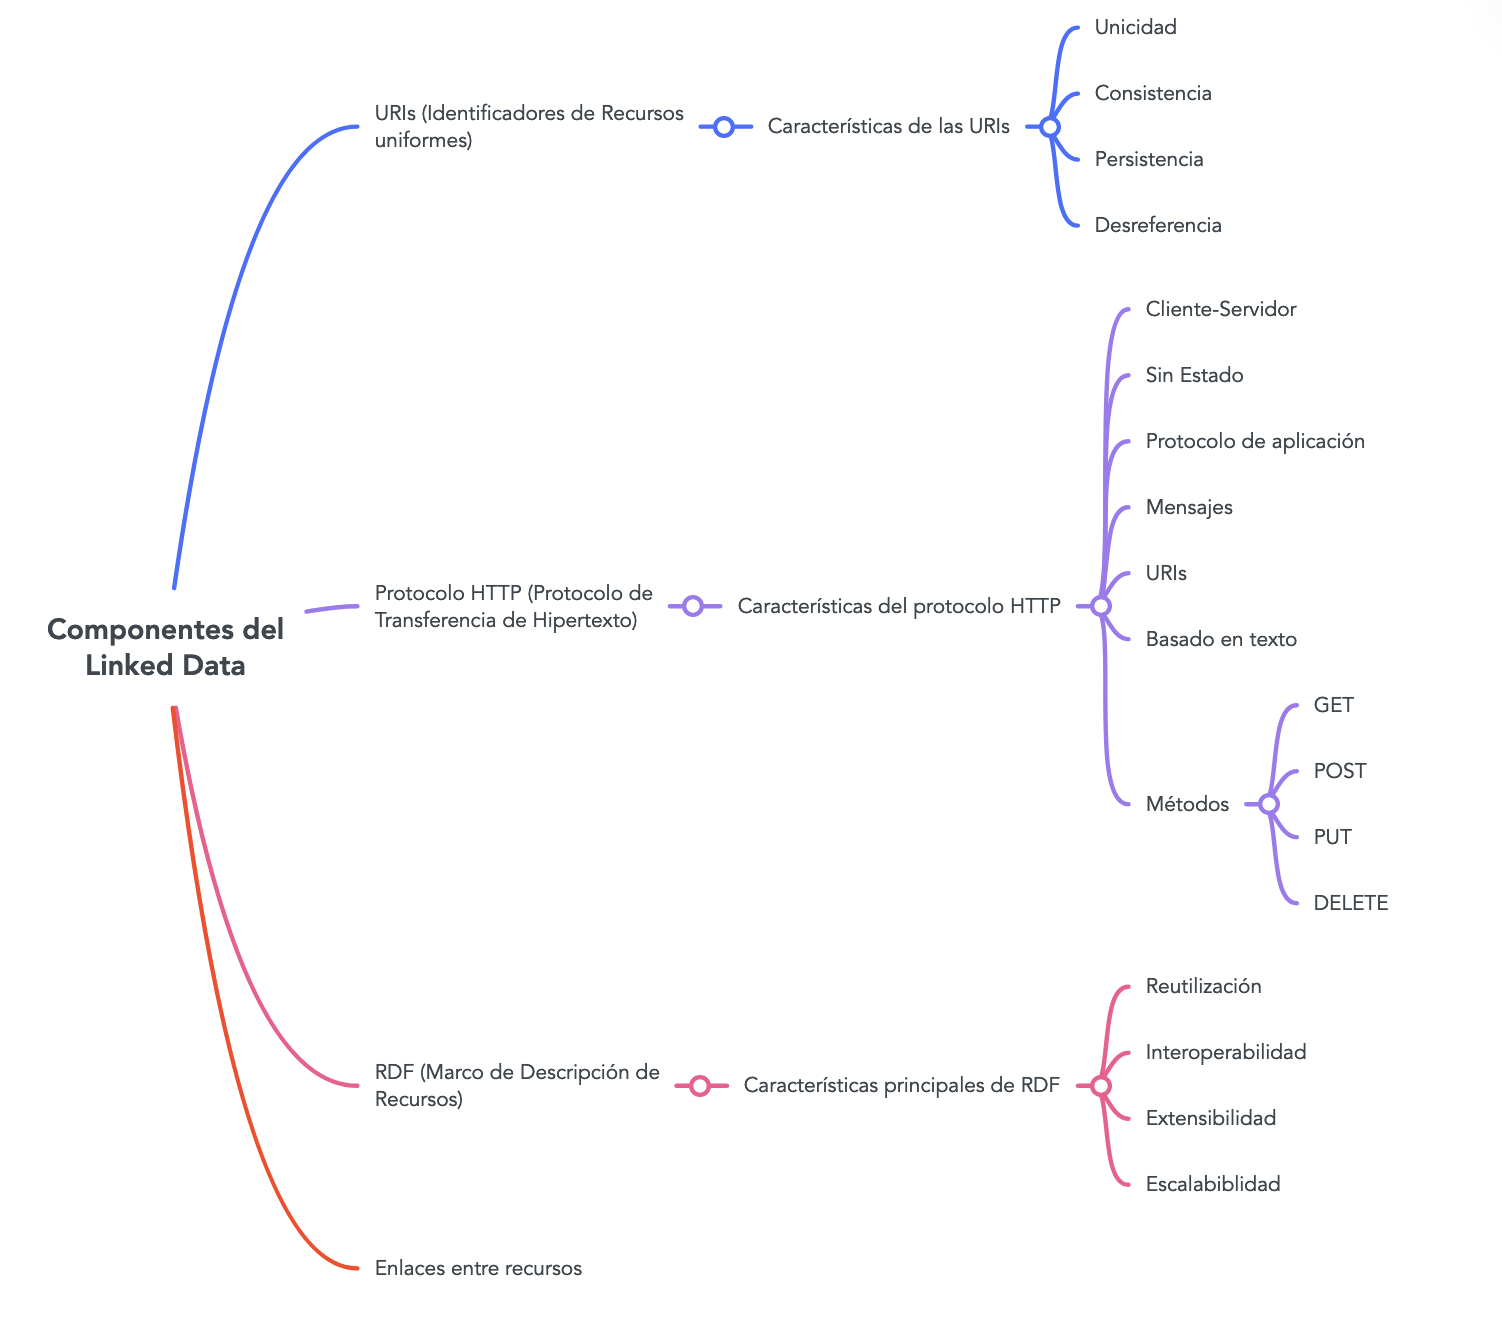
\includegraphics[scale=0.6]{../img/Componentes-Linked-Data.png}
	\caption{Esquema de los principales componentes de Linked Data..}
	\label{fig:Componentes-Linked-Data}
\end{figure}

\chapter{URI}

\section{Introducción a las URIs}

Una \textbf{URI} (identificador uniforme de recursos). se utilizan en una gran variedad de contexto, ya sea en la WWW, en la mensajería electrónica y en los sistemas de archivos. En dicho sentido se dice que las URIs son identificadores de recursos uniformes. La sintaxis básica de una URI se compone de los siguiente elementos:

- \textbf{Esquema}: Se trata de la parte inicial de la URI, la cual, se trata de un identificador de esquema que se utiliza para identificar el tipo de recurso que se está identificando. Por ejemplo, en el caso de las URIs de la web, el esquema es \texttt{http} o \texttt{https}.

- \textbf{Autoridad}: Se trata de la parte de la URI que identifica la autoridad que controla el recurso. En el caso de las URIs de la web, la autoridad es el nombre de dominio. Por ejemplo:

Se tiene la siguiente URI tomada como ejemplo:

\begin{verbatim}
	https://www.example.com/index.html
\end{verbatim}

\fbox{\parbox{\textwidth}{
		\textbf{Autoridad}: www.example.com
	}}

- \textbf{Parámetros}: Se trata del fragmento que se encarga de proporcionar información adicional sobre los recursos. Por ejemplo:

Se hace uso de una URI similar a la adjunta anteriormente:

\begin{verbatim}
	https://www.example.com/index.html?lang=es
\end{verbatim}

\fbox{\parbox{\textwidth}{
		\textbf{Parámetros}: lang=es
	}}

- \textbf{Fragmento}: se trata del segmento que trata de identificar una parte específica del recurso. Por ejemplo:

Finalmente se tiene la siguiente URI tomada como muestra:

\begin{verbatim}
	https://www.example.com/index.html#section1
\end{verbatim}

\fbox{\parbox{\textwidth}{
		\textbf{Fragmento}: section1
	}}

\section{Diferencias entre URI y URL}

Como se ha podido ver en la sección anterior, podemos considerar que las URIs y las URLs \texttt{(Uniform Resource Locator)} son lo mismo y que son iguales, pero, no son lo mismo, ya que, una URLse utiliza 
\begin{wrapfigure}{r}{0.30\textwidth}
	
	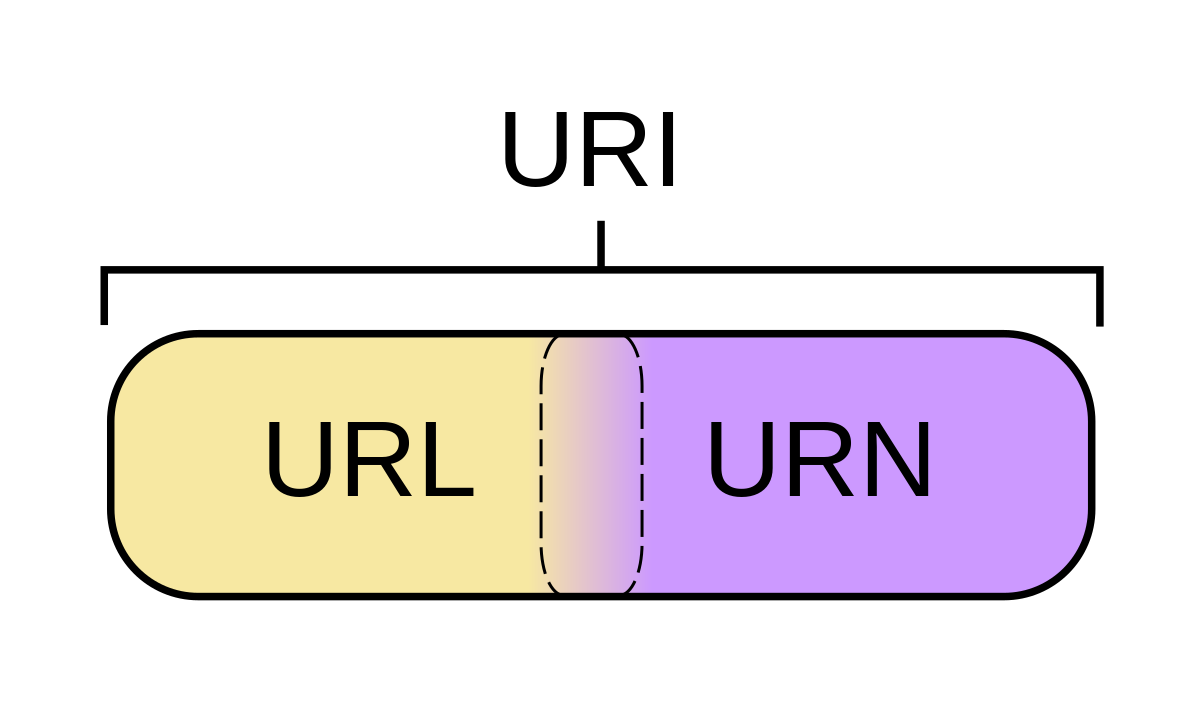
\includegraphics[width=0.25\textwidth]{../img/uri.png}
	\caption{URI vs URL.}
	\label{fig:Uri}
\end{wrapfigure}
de manera principal para apuntar una página web o una parte de estas, haciendo uso de esquemas o protocolos como http, https o ftp, permitiendo mejorar la facilidad con la que se puede acceder a las ubicaciones de los distintos recursos que existen en la web. Por otro lado, una URI se utiliza para definir las identidades de los objetos, de manera independiente del método que se use. 

Con todo esto comentado anteriormente, se puede afirmar que una URL se trata de una URI o de un tipo de URI, pero, no se puede decir que una URI puede ser una URL.

Para poder comprender un poco mejor la diferencia entre una URL y una URI, se puede observar la siguiente imagen \ref{fig:URI-URL}.

\begin{figure}[H]
	\centering
	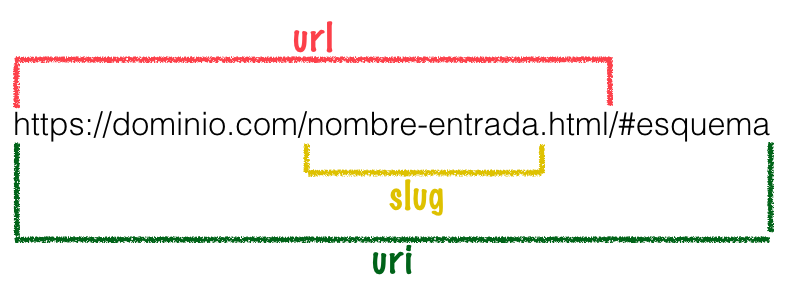
\includegraphics[scale=0.6]{../img/diferencia-entre-url-y-uri.png}
	\caption{Diferencia entre URI y URL.}
	\label{fig:URI-URL}
\end{figure}

\fbox{\parbox{\textwidth}{
		\textbf{Nota}: el termino \texttt{slug} que se puede observar en la imagen identifica el contenido específico de una página, es decir, se utiliza para describir el contenido de la página de manera que sea fácil de entender por parte del usuario final.
	}}

\section{Tipos de URI}

Para finalizar con esta sección, se puede hablar de los distintos tipos de URIs que existen:

- \textbf{IRI}: Se trata del identificador internacional de recursos. Es decir, se trata de una versión internacionalizada de las URIs. Esto quiere decir que, se trata de una URI que puede contener caracteres Unicode, al contrario que la URI que solo admite la codificación ASCI.

- \textbf{URL}: Se trata del identificador uniforme de recursos, consiste en una URI que indica la ubicación de un recurso en internet, permitiendo localizarlo de manera sencilla.

- \textbf{URN}: Se trata del nombre uniforme de recursos, consiste en una URI que identifica de manera única un recurso, pero, no indica su ubicación. Por tanto, indica un nombre único y público de un recurso en internet.

- \textbf{URC}: Se trata de la citación uniforme de recursos, es decir, se trata de una URI que se utiliza para citar un recurso en internet.

\chapter{HTTP}

\section{Introducción a HTTP}

HTTP \texttt{Protocolo de Transferencia de Hipertexto en español} es un protocolo de la capa de aplicación del modelo OSI, que se encarga de la transmisión de documentos como HTML.  Dicho protocolo se basa en el modelo cliente servidor, donde un cliente puede realizar solicitudes y un servidor se encarga de dar respuestas a dichas solicitudes. Cada recurso que se encuentran dentro de la web, ya sean páginas web, imágenes, documentos, etc, es identificado por una URL y puede ser accedido a través de las distintas solicitudes que proporciona el protocolo HTTP.

Teniendo en cuenta el contexto de \textbf{Linked Data}, se puede decir que HTTP es el protocolo de la web, ya que, este permite cumplir con la filosofía que sigue Linked Data, ya que esta busca publicar y conectar datos en la web de tal manera que se encuentren interconectados y puedan ser consultados de forma coherente.

\section{HTTP y Linked Data}

HTTP se utiliza para poder acceder a los recursos de datos que se encuentran en la web, estos, se identifican mediante URI. Es por ello que, las URI de Linked Data suelen utilizar el esquema "http" o "https" para poder identificar los recursos comentados. Para poder comprender todo esto se puede observar el siguiente ejemplo de URI que permite la identificación de un recurso de datos sobre el pueblo de Tinajo en Lanzarote.

\begin{verbatim}
	http://datos.tinajo.es/resource/poblacion/2019
\end{verbatim}

La URI adjunta permite que mediante una solicitud \textbf{HTTP GET} se puedan acceder a los datos que existen sobre la población de Tinajo en Lanzarote en el año 2019. De esta manera, HTTP permite la recuperación de recursos en la web. Por otro lado, HTTP también permite publicar datos de Linked Data en la web mediante un servidor HTTP, dicho servidor, puede responder a las distintas solicitudes de los clientes o de aquellos usuarios que quieran acceder a los recursos. Un ejemplo de implementación de servidor que permita publicar el recurso de la población de Tinajo en Lanzarote en el año 2019.

\begin{verbatim}
	# Librerías necesarias
	import requests
	import json

	# Definición de la URI del recurso
	uri = "http://datos.tinajo.es/resource/poblacion/2019"

	# Definición de los datos del recurso
	data = {
			"name": "Tinajo",
			"population": 6.000,
			"capital": False
	}

	# Publicación de los datos mediante una solicitud \textbf{POST HTTP}
	requests.post(uri, data=json.dumps(data))
\end{verbatim}

El código permite crear un nuevo recurso sobre Tinajo en el servidor HTTP, teniendo en cuenta los siguientes datos:

- El nombre del recurso es Tinajo.

- La población de Tinajo es de 6.000 habitantes.

- Tinajo no es la capital de Lanzarote.

\section{implementación de Linked Data con HTTP}

Dentro de la implementación de Linked Data haciendo uso del protocolo HTTP se deben de seguir una serie de pasos que permiten la correcta implementación de este. Por tanto, se puede hablar de los siguientes pasos:

1. Identificación de los distintos recursos de datos.

2. Asignación de URIs a cada uno de los recursos.

3. Publicación de los datos de los recursos en la web.

\subsection{Identificación de Recursos}

En cuanto a la identificación de los distintos recursos de datos se debe de seguir una metodología que va desde el análisis del contenido de los distintos documentos HTML hasta la utilización de un vocabulario de Linked Data.

\subsection{Asignación de URIs}

Tras la identificación de los distintos recursos de datos se procede a la asignación de URIs a cada uno de los recursos. Para ello, se debe de tener en cuenta que las URIs deben de ser únicas, persistentes y desreferenciables. Para ello se debe de hacer uso de un esquema de URI que se encuentre predefinido \cite{16} o la creación de una URI personalizada.

\subsection{Publicación de los datos}

Para finalizar, se debe de publicar los datos de los recursos en la web. Para ello, se debe de hacer uso de un servidor HTTP que permita la publicación de los datos de los recursos. Además, se debe de tener en cuenta que los datos deben de ser publicados en un formato estándar como RDF, JSON-LD, Turtle, etc. A pesar de ello, el formato que se hace uso para Linked Data en este caso es RDF.

\chapter{RDF}

\section{Introducción a RDF}

Como se ha comentado de manera previa, \texttt{RDF} es un \textbf{modelo} que permite representar propiedades y valores de propiedades. Este, se basa en principios que se encuentran establecidos haciendo uso de varios tipos de representación de datos. Por otro lado, se puede hablar de las \textbf{propiedades RDF}, estas, se asemejan a los atributos y de manera general se corresponden con los pares de atributo-valor. Por último, se puede hablar de los \textbf{recursos RDF}, estos, se asemejan a los objetos en cuanto a aspectos de la terminología del diseño orientado a objetos, por tanto, los \texttt{recursos} son los objectos y las \texttt{propiedades} son los objetos específicos y variables de una categoría.

\section{Modelo de datos RDF}

En cuanto al modelo de datos básico de \textbf{RDF} se basa en los siguientes tres tipos de objetos:

- \textbf{Recursos}: Los recursos se tratan de los objetos que se quieren describir, es decir, se enfocan como todos los elementos que son descritos por expresiones RDF. Es decir, por ejemplo, un recurso puede se una página web completa, una parte de una página web, una colección completa de páginas, etc. Para finalizar, los recursos se deben de designar siempre por URIs más etiquetas de identificación de destino.

- \textbf{Propiedades}: Las propiedades se tratan de los atributos que se quieren describir, es decir, se trata de un aspecto específico, característica, atributo o relación utilizado para describir un recurso. Por ejemplo, una propiedad puede ser el título de una página web, el autor de una página web, la fecha de creación de una página web, etc.  Cada propiedad tiene un significado en específico, define los valores permitidos, los tipos de recursos que puede describir y las relaciones con otras propiedades.

- \textbf{Sentencias}: Las sentencias se tratan de una expresión que relaciona un recurso con una propiedad y un valor. Las tres partes individuales de una sentencia se denominan como \textbf{sujeto (\texttt{recurso}), predicado (\texttt{propiedad}) y objeto (\texttt{valor de la propiedad o literal})}, es decir, los denominados \textbf{tripletes}. El objeto de una sentencia puede ser otro recurso o un valor literal, a su vez un recurso puede ser especificado por un URI o una cadena simple de caracteres que se denominan como \textbf{literales}, además, dicho recurso puede ser a su vez datos primitivos definidos por \textbf{XML} (Lenguaje de marcado extensible) \cite{6}.

\section{Ejemplos de sentencias RDF}
Para poder comprender todo esto anterior, se tiene el siguiente ejemplo de sentencia RDF:

\begin{verbatim}
	http://www.example.es/index.html tiene una desarrolladora cuyo valor es Andrea López.
\end{verbatim}

\begin{quote}
	\textbf{Sujeto}: http://www.example.es/index.html

	\textbf{Predicado}: "desarrollador"

	\textbf{Objeto}: Andrea López
\end{quote}

Tras esto, se puede observar el diagrama de nodo y arco simple que representa el ejemplo adjunto anteriormente:

\begin{figure}[H]
	\centering
	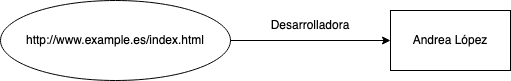
\includegraphics[scale=0.7]{../img/Diagrama-Nodo-Arco.png}
	\caption{Diagrama de nodo y arco simple que representa el ejemplo de sentencia RDF.}
	\label{fig:Diagrama-Nodo-Arco}
\end{figure}

\fbox{\parbox{\textwidth}{
		\textbf{Nota:} La dirección de la flecha del arco simple es muy importante. El arco siempre debe de empezar en el sujeto y apunta hacia el objeto de la sentencia RDF. De manera general se puede usar la siguiente sentencia:

		\textbf{<Sujeto> TIENE <Predicado> <Objeto>}
	}}

A partir del ejemplo comprendido de manera previa, se pueden especificar algunas características más para dicho ejemplo como:

\begin{verbatim}
	El individuo cuyo nombre es Andrea López, correo electrónico <andre@example.es>, 
	es la desarrolladores de la página web <http://www.example.es/index.html>.
\end{verbatim}

Teniendo esto en cuenta, la intención del ejemplo se basa en darle valor a la propiedad \textbf{desarrolladora} mediante una entidad estructurada. Por tanto, se puede observar a continuación el diagrama de nodo y arco simple que representa el ejemplo adjunto anteriormente:

\begin{figure}[H]
	\centering
	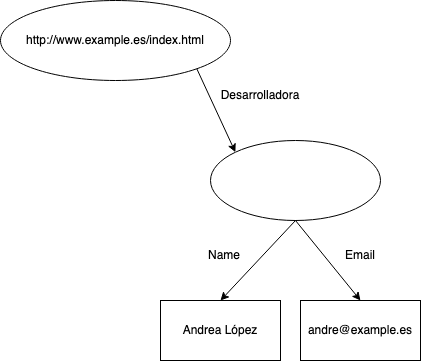
\includegraphics[scale=0.7]{../img/Propiedad-Estructurada.png}
	\caption{Diagrama de nodo y arco simple que representa el ejemplo de sentencia RDF.}
	\label{fig:Diagrama-Nodo-Arco-2}
\end{figure}

\fbox{\parbox{\textwidth}{
		\textbf{Nota:} Se puede leer el diagrama anterior como http://www.example.es/index.html tiene la desarrolladora cualquiera y este cualquiera tiene el nombre Andrea López y el correo electrónico andre@example.es .
	}}

Para finalizar, se puede implementar como ejemplo el uso de múltiples frases o sentencias RDF, por tanto, se tiene el siguiente ejemplo para ello:

\begin{verbatim}
	El individuo al que se refiere el identificador de empleado id 15151 se llama Andrea López y 
	tiene la dirección de correo electrónico <andre@example.es>. Este individuo creó el 
	recurso <http://www.example.es/index.html> y es la desarrolladora de este recurso.
\end{verbatim}

Con esto en mente, se implementad el siguiente \textbf{modelo RDF}:

\begin{figure}[H]
	\centering
	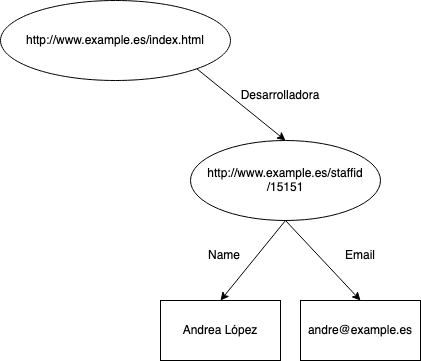
\includegraphics[scale=0.7]{../img/Modelo-RDF.png}
	\caption{Modelo RDF que representa el ejemplo de múltiples sentencias RDF.}
	\label{fig:Modelo-RDF}
\end{figure}

\chapter{RDF y XML}

\section{comparación entre RDF y XML}

Para comenzar con esta sección,  se establecerá una comparación entre \texttt{RDF} y \texttt{XML}. RDF hace uso del lenguaje XML \textbf{(Extensible Markup Language)} como método para poder representar la información.

XML no se trata de un lenguaje de etiquetado, sino que se trata de un \textbf{Metalenguaje}, es decir, de un lenguaje que establece un conjunto de reglas que permiten a su vez la creación de lenguajes de etiquetado. Es decir, XML de manera única muestra las distintas normas que se deben de seguir sobre cómo se combinan las cadenas de caracteres, cómo se tienen de que especificar las propiedad de los elementos, etc.

Es por ello que, tras entender el concepto de XML, se puede comentar que RDF hace uso de una DTD \textbf{(Document Type Definition)} de XML para desarrollar las propias etiquetas de RDF, es decir, una DTD se trata de un documento específico de trabajo dónde se establece un esquema el cuál nos permite informar sobre el contenido de cada conjunto de datos, la interpretación de estos y la forma correcta de trabajar con ellos. De esta manera, RDF al hacer uso de XML se favorece a la hora de generar nuevos conjuntos de etiquetas y el mecanismo semántico que ofrece para expresar la descripción de cualquier tipo de recurso RDF.

Por otra parte, XML permite la generación de árboles con los distintos elementos y subelementos que forman el documento, a la vez, permite la representación del documento añadiendo o eliminando etiquetas.

\section{Estructura del documento XML}

Un documento XML debe de incluir un \textbf{prólogo} y la \textbf{instancia documento}. El \texttt{prólogo} está formado por tres secciones distintas:

- Declaración XML.

- Declaración del tipo de documento.

- Referencia a una hoja de estilo externa.

Por tanto, para la comprensión de las distintas partes en las que se divide el documento XML se puede observar el siguiente ejemplo para ello:

\begin{verbatim}
		<?xml version="1.0" encoding="ISO-8859-1" standalone="no"?>
		<!DOCTYPE ProductoElectronico SYSTEM "producto.dtd">
		<?xml-stylesheet href="productohtml.xsl" type="text/xsl"?>
		<TiendaElectronica>
			<ProductoElectronico>
				<Nombre>Smartphone Galaxy</Nombre>
				<Marca>Samsung</Marca>
				<Precio>599.99</Precio>
			</ProductoElectronico>
			<ProductoElectronico>
				<Nombre>Portátil Inspiron</Nombre>
				<Marca>Dell</Marca>
				<Precio>799.99</Precio>
			</ProductoElectronico>
		</TiendaElectronica>
	\end{verbatim}

Teniendo en cuenta el ejemplo adjunto anteriormente, se puede observar en la siguiente imagen \ref{fig:Example-XML} las distintas partes en las que se divide el prólogo en XML.

\begin{figure}[H]
	\centering
	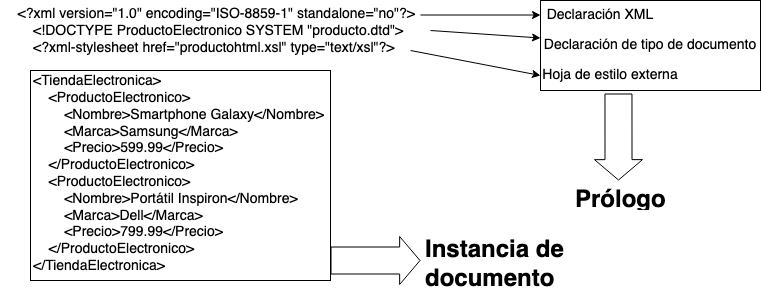
\includegraphics[scale=0.7]{../img/XML-Example-1.png}
	\caption{Esquema de partes en las que se divide el documento XML.}
	\label{fig:Example-XML}
\end{figure}

\chapter{Tim Berners-Lee}

\section{Principios de Linked Data según Tim Berners-Lee}

Tras comprender un poco más sobre los aspectos básicos de \texttt{Linked Data} durante los cuatro capítulos desarrollados anteriormente, podemos hablar de \textbf{Tim Berners-Lee } \cite{11}, el padre de la web,  el cual, en la presentación sobre Linked Data en las conferencias TED 2009, explicó los principios de linked data mediante tres reglas que permiten entender el concepto de esto de una manera mucho más sencilla:

1. Todos los objetos conceptuales posee denominaciones que se inician con HTTP.

2. Si se toma uno de los nombres HTTP y se realiza una búsqueda, se recibirá como resultado ciertos datos en un formato estándar que resulta útil para aquel que quiera conocer sobre dicha cosa o evento.

3. Cuando se obtiene información, no sólo se obtiene la información que se buscaba, sino que también se obtiene información sobre otros objetos relacionados con el objeto que se buscaba, es decir, sus relaciones. Y, cuando existen relaciones, a pesar de que no se trata de la información que se buscaba, esos propios datos también tendrán nombre que empiezan por HTTP, por tanto, se podrá acceder a ellos de la misma manera que se accedió a la información que se buscaba en un principio.

Con esto, la plataforma de Datos Enlazados \textbf{(LDP, Linked Data Plataform)} define una serie de reglas para las distintas operaciones HTTP sobre los recursos web, algunos de estos están basados en \texttt{RDF}, permitiendo promover una arquitectura para leer y escribir Datos Enlazados en la web.

\chapter{Linked Data Plataform, LDP}
SAMUEL

\chapter{Linked Open Data (LOD)}
		\begin{wrapfigure}{r}{0.30\textwidth}
			\centering
			\includegraphics[width=0.25\textwidth]{../img/W3C®_Icon.svg.png}
			\caption{(World Wide Web).}
			\label{fig:od->W3C}
		\end{wrapfigure}
		Linked Open Data (LOD), o Datos Vinculados Abiertos en español, representa un conjunto de prácticas fundamentales para la publicación y conexión de datos estructurados en la World Wide Web. La premisa central de LOD es hacer que los datos estén disponibles de una manera que facilite su acceso, búsqueda y reutilización, fomentando así la interconexión de conjuntos de datos diversos. Estas prácticas se respaldan en estándares internacionales establecidos por el World Wide Web Consortium (W3C).
		
		LOD encuentra sus raíces en la necesidad de superar los desafíos asociados con la diversidad de formatos de datos en la web, que incluyen archivos como PDF, TIFF, CSV y documentos de Word. Aunque estos datos son accesibles a través de enlaces HTML, su procesamiento automatizado a menudo requiere esfuerzos adicionales debido a la falta de estructura semántica.

		\section{Principios Clave de LOD}

		La implementación de LOD busca establecer una forma universal para que cualquier persona pueda leer, compartir y reutilizar datos en la web. La clave para esto es la interrelación de datos, donde diferentes conjuntos de datos están enlazados entre sí, permitiendo una mayor eficiencia en la búsqueda y utilización de información.

		\section{Beneficios de LOD}

		La adopción de LOD conlleva varios beneficios, incluyendo:

		\begin{itemize}
		\item \textbf{Accesibilidad Mejorada:} Al seguir estándares y principios de LOD, se mejora la accesibilidad de los datos, permitiendo su fácil recuperación y uso.
		
		\item \textbf{Eficiencia en la Búsqueda:} La interconexión de datos en LOD facilita la búsqueda y recuperación de información de manera más eficiente.
		
		\item \textbf{Reutilización de Datos:} LOD fomenta la reutilización de datos al establecer un marco que facilita compartir y combinar conjuntos de datos de manera significativa.
		
		\item \textbf{Aplicaciones Interconectadas:} La interrelación de datos en LOD facilita la creación de aplicaciones interconectadas que pueden aprovechar la diversidad de información disponible en la web.
		\end{itemize}

		\begin{figure}[H]
			\centering
			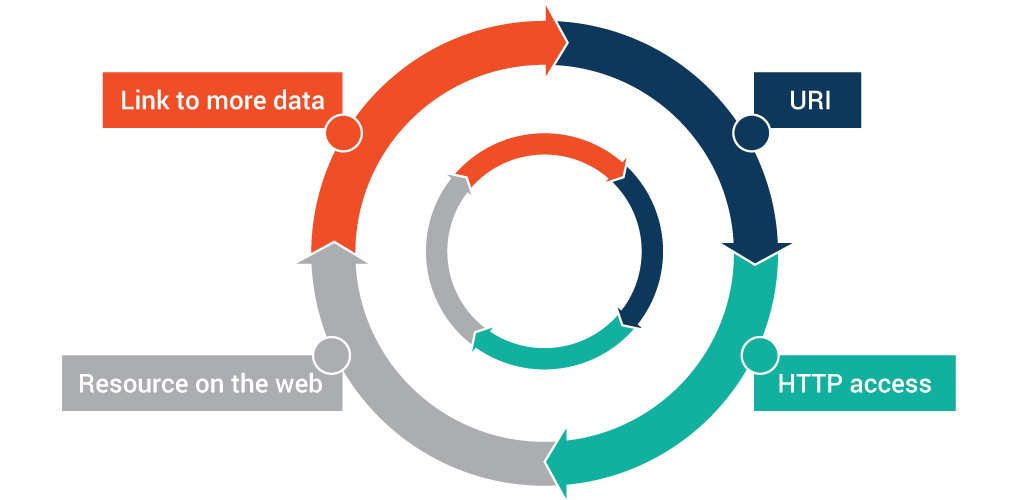
\includegraphics[scale=0.2]{../img/What-are-Linked-Data-and-Linked-Open-Data.png}
			\caption{Linked Data y Linked Open Data.}
			\label{fig:LOD}
		\end{figure}


	\chapter{Relación entre Linked Data y Open Data}

		La relación entre Linked Data y Open Data es esencial para comprender cómo la combinación de estos enfoques puede potenciar la gestión y la utilidad de los conjuntos de datos. A continuación, se profundizará en algunos aspectos clave de esta relación:
		
		\subsection*{10.1 Interoperabilidad y Enlace de Datos}
\begin{itemize}
  \item Facilita Conexiones: Combinar Linked Data y Open Data simplifica la vinculación de diversos conjuntos de datos.
  \item Mecanismo Central: Linked Data enfoca la creación de enlaces mediante identificadores únicos (URI), estableciendo puntos de conexión consistentes.
  \item Impacto General: Favorece la interacción entre sistemas y aplicaciones, promoviendo un ecosistema de datos más amplio y conectado.
\end{itemize}
\begin{figure}[H]
	\centering
	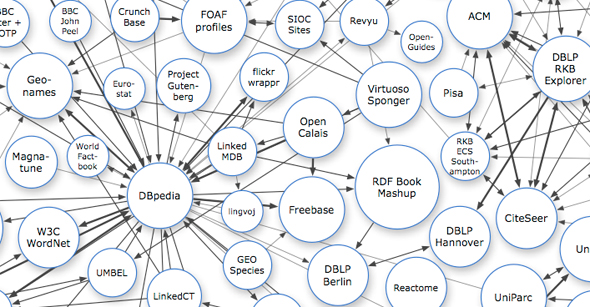
\includegraphics[scale=0.4]{../img/lod.jpg}
	\caption{LOD Cloud.}
	\label{fig:lod}
\end{figure}

\subsection*{10.2 Descubrimiento y Explotación de Datos}
\begin{itemize}
  \item Oportunidades Innovadoras: La fusión de Linked Data y Open Data abre nuevas posibilidades para el descubrimiento y la explotación de datos.
  \item Enfoque Eficiente: Utilizando identificadores únicos y estándares semánticos, es posible descubrir relaciones y patrones complejos, especialmente valioso en contextos científicos y empresariales.
\end{itemize}
\subsection*{10.3 Transparencia y Confianza en los Datos}
\begin{itemize}
  \item Fortalecimiento de la Transparencia: Linked Data refuerza la transparencia en Open Data al proporcionar una estructura semántica clara.
  \item Seguimiento de Relaciones: Al enlazar efectivamente conjuntos de datos abiertos, se pueden seguir relaciones entre entidades, fortaleciendo la confianza en cómo se recopilaron y relacionaron los datos.
\end{itemize}

\subsection*{10.4 Potencial para la Innovación y la Creación de Valor}
\begin{itemize}
  \item Entorno Propicio: La combinación de Linked Data y Open Data crea un entorno favorable para la innovación y la creación de valor.
  \item Oportunidades Generadas: Permite a desarrolladores e investigadores acceder y vincular datos eficientemente, generando oportunidades para la inteligencia artificial, la ciencia de datos y la toma de decisiones basada en datos.
\end{itemize}
\subsubsection{Veamos un Ejemplo Práctico: Sistema de Transporte Urbano}

En una ciudad, los datos sobre horarios de autobuses, rutas, paradas y disponibilidad en tiempo real se publican como Open Data, siguiendo los principios de Linked Data. Veamos cómo este enfoque beneficia tanto a los ciudadanos como a los desarrolladores:

\begin{itemize}
    \item \textbf{Descubrimiento Eficiente:} Los ciudadanos pueden acceder fácilmente a los horarios de autobuses y rutas mediante aplicaciones de terceros que aprovechan los datos abiertos. Esto facilita la planificación de viajes y reduce el tiempo de espera en las paradas.
    
    \item \textbf{Desarrollo de Aplicaciones Innovadoras:} Los desarrolladores pueden crear aplicaciones que combinan datos de transporte con información meteorológica y eventos locales. Por ejemplo, una aplicación podría sugerir rutas alternativas en caso de eventos especiales o condiciones climáticas adversas.
    
    \item \textbf{Identificación de Patrones de Uso:} Gracias a la interconexión de datos, las autoridades de transporte pueden analizar patrones de uso, identificar áreas con alta demanda y ajustar eficientemente los servicios para satisfacer las necesidades de la comunidad.
\end{itemize}
\begin{figure}[H]
	\centering
	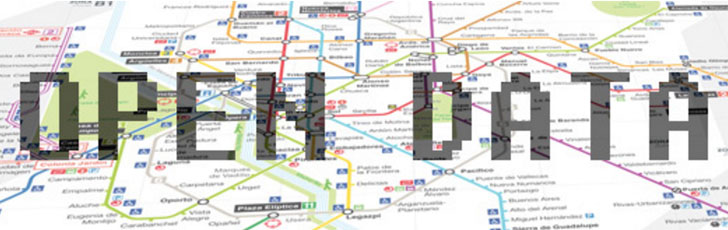
\includegraphics[scale=0.4]{../img/transport.jpg}
	\caption{Red Transporte Abierta.}
	\label{fig:opendata}
\end{figure}

Este ejemplo ilustra cómo la combinación de Linked Data y Open Data en el contexto del transporte urbano no solo facilita el acceso a la información, sino que también fomenta la innovación y mejora la eficiencia en la gestión de servicios públicos.


\subsection*{10.5 Desafíos y Consideraciones Éticas}
\begin{itemize}
  \item Consideraciones Críticas: A pesar de los beneficios, la convergencia de datos plantea desafíos, especialmente en términos de privacidad y seguridad.
  \item Acciones Necesarias: Implementar medidas de seguridad robustas y abordar preocupaciones éticas es esencial para garantizar la apertura e interconexión de datos sin comprometer la privacidad ni generar riesgos indebidos.
\end{itemize}
		
		Aunque la convergencia de Linked Data y Open Data ofrece beneficios significativos, también plantea desafíos. La privacidad y la seguridad son consideraciones críticas, especialmente en el caso de datos abiertos enlazados. Es esencial implementar medidas de seguridad robustas y abordar las preocupaciones éticas para garantizar que la apertura y la interconexión de datos no comprometan la privacidad de las personas ni generen riesgos indebidos.
	\chapter{Linked Data y Web Semántica}
	LOD se apoya en la web semántica, la cual es
	una web que permite a las máquinas leer y
	compartir información, donde cada fuente de
	datos puede ser usada en diferentes aplicaciones. 
	En el continuo desarrollo de la web, dos conceptos fundamentales han surgido como pilares para la construcción de una web más inteligente y significativa: Linked Data y Web Semántica. Este informe explora la relación intrínseca entre estos dos conceptos, resaltando sus roles individuales y cómo, en conjunto, contribuyen a una web más conectada y rica en significado.
	
	\section{Web Semántica: Dando Significado a los Datos}
	
	La Web Semántica es una extensión de la web actual que busca agregar un nivel de significado a la información, permitiendo a las máquinas comprender y procesar datos de manera más inteligente. Algunas características clave de la Web Semántica son:
	
	\begin{enumerate}
		\item \textbf{Lenguajes Semánticos:} Uso de estándares como RDF y OWL para representar información de manera semántica.
	   
		\item \textbf{Interconexión de Datos:} Enlazar datos de manera que las relaciones sean comprensibles tanto para humanos como para máquinas.
		
		\item \textbf{Agentes Inteligentes:} Máquinas capaces de razonar sobre datos y realizar tareas más complejas.
	\end{enumerate}
		
	\begin{figure}[H]
		\centering
		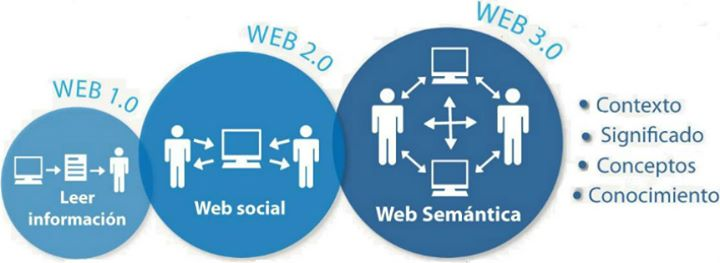
\includegraphics[scale=0.4]{../img/websemantica.jpg}
		\caption{Relación entre Linked Data y Web Semántica.}
		\label{fig:websemantica}
	\end{figure}

	La \textbf{Web Semántica} busca enriquecer los datos al agregar capas de significado semántico. Esto se logra mediante el uso de estándares como \textbf{RDF} (Resource Description Framework) y \textbf{OWL} (Web Ontology Language), que permiten representar relaciones y significados de manera formal y estructurada.

	\section{Interoperabilidad entre Aplicaciones}

	Un objetivo clave de la \textbf{Web Semántica} es mejorar la interoperabilidad entre aplicaciones y sistemas. Al utilizar estándares semánticos, los datos se vuelven más comprensibles para las máquinas, lo que facilita la integración y el intercambio de información entre diferentes plataformas.

	\section{Descubrimiento de Conocimiento}

	La \textbf{Web Semántica} permite un mejor descubrimiento de conocimiento al facilitar la identificación de patrones y relaciones en los datos. Al agregar semántica a los datos, se mejora la capacidad de las máquinas para inferir información y descubrir conocimiento implícito.

	\section{Agentes Inteligentes y Automatización}

	La presencia de agentes inteligentes, impulsados por la semántica de los datos, permite la automatización de tareas más complejas. Estos agentes pueden razonar sobre la información, realizar consultas avanzadas y ejecutar acciones basadas en reglas semánticas predefinidas.

	\section{Búsqueda Semántica}

	La \textbf{Web Semántica} impulsa el desarrollo de motores de búsqueda semántica, que van más allá de la coincidencia de palabras clave y comprenden el significado detrás de las consultas. Esto mejora la precisión de los resultados de búsqueda al considerar el contexto semántico de la información.

	\section{Evolución hacia la Web 3.0}

	A menudo, se asocia la \textbf{Web Semántica} con la transición hacia la \textbf{Web 3.0}, que representa la próxima fase de la evolución de la web. La \textbf{Web 3.0} se caracteriza por una web más inteligente, descentralizada y orientada a la semántica, donde las máquinas pueden comprender y utilizar el contenido de manera más eficiente.

	\section*{Integración de Linked Data y Web Semántica}
	
	La relación entre Linked Data y Web Semántica es de complementariedad. Linked Data establece la estructura y la interconexión, mientras que la Web Semántica agrega capas de significado para una comprensión más profunda. Puntos clave de integración incluyen:
	
	\begin{enumerate}
		\item \textbf{Contextualización Semántica:} La Web Semántica aporta capas de significado a los datos vinculados, mejorando su comprensión y utilidad.
		
		\item \textbf{Agentes Inteligentes en Datos Conectados:} La presencia de agentes inteligentes se beneficia enormemente de la estructura y la interconexión proporcionadas por Linked Data.
		
		\item \textbf{Interoperabilidad Mejorada:} La combinación de Linked Data y Web Semántica impulsa la interoperabilidad, facilitando el uso conjunto de datos heterogéneos.
	\end{enumerate}
	
	\section*{Desafíos y Consideraciones}
	
	Aunque la integración de Linked Data y Web Semántica ofrece beneficios sustanciales, también presenta desafíos. La estandarización de ontologías, la privacidad y la seguridad son consideraciones críticas que deben abordarse para garantizar un desarrollo ético y sostenible.
	
	\chapter{Transformación de open data a linked open data}
		  \subsection*{Paso 1: Identificación de Datasets}

		  \begin{itemize}
			\item \textbf{Definir Contenido:} Determine el contenido específico que desea publicar como Linked Open Data (LOD).
			
			\item \textbf{Formatos de Datos:} Identifique los formatos en los que se encuentran los datos, como formatos tabulares, CSV, JSON, entre otros.
			
			\item \textbf{Colaboradores:} Identifique a los colaboradores involucrados en el proceso de transformación y publicación de datos enlazados.
			
			\item \textbf{Entidades Externas:} Identifique entidades externas con las que podría enlazar los datos para enriquecer su contexto.
			
			\item \textbf{Diseño de URIs:} Diseñe URIs para la identificación y localización de los datos. Asegúrese de que estas URIs sean únicas y descriptivas.
		\end{itemize}	
		\subsection*{Paso 2: Limpieza de Datos}
			\begin{itemize}
			\item \textbf{Realizar Correcciones:} Limpieza de errores ortográficos, vacíos, formatos y caracteres innecesarios.
			
			\item \textbf{Calidad de Datos y Metadatos:} Asegúrese de que los datos cumplan con los estándares de calidad y metadatos.
			\end{itemize}		
		\subsection*{Paso 3: Modelado de Datos}
		\begin{itemize}
			\item \textbf{Determinar un Modelo de Datos RDF:} Identifique el modelo de datos RDF que mejor se adapte a sus necesidades, como RDF, RDF Schema, OWL, entre otros.
			
			\item \textbf{Seleccionar Datos Relevantes:} Seleccione los datos relevantes para el modelo de datos RDF seleccionado.
			
			\item \textbf{Identificar Tripletas:} (Objeto, predicado, sujeto) en los datos.
			
			\item \textbf{Reutilizar Vocabularios Existentes:} Aproveche vocabularios existentes y defina aquellos que se utilizarán, como Dublin Core, FOAF, Schema.org, entre otros.
		\end{itemize}
		
		\subsection*{Paso 4: Enriquecimiento de Datos}
		\begin{itemize}
			\item \textbf{Conocimiento Acumulado:} de datos, vocabularios y ontologías.
			
			\item \textbf{Visión General de Ontologías:} Disponibles y apropiadas para el dominio de los datos.
			
			\item \textbf{Enriquecer el RDF con Ontologías:} Mediante enlaces. Repita los pasos 2 y 3 si la información es útil.
			
			\item \textbf{Modelo RDF Final:}
		\end{itemize}
		\subsection*{Paso 5: Vinculación de Datos}
		\begin{itemize}
			\item \textbf{Seleccionar el Método más Apropiado:} Para convertir los datos enlazados a RDF.
			
			\item \textbf{Convertir los Datos:}
		\end{itemize}
		\subsection*{Paso 6: Publicación de Datos}
		\begin{itemize}
			\item \textbf{Seleccionar Posibilidades:} Para publicar LOD.
			
			\item \textbf{Conceptos Básicos:} De Triplestore y SPARQL.
			
			\item \textbf{Evaluar:} Posibilidad más adecuada para el paso 4.
			
			\item \textbf{Publicar LOD:}
		\end{itemize}
		\subsection*{Paso 7: Validación de Datos}
		\begin{itemize}
			\item \textbf{Conjuntos de Datos Candidatos:} Para la próxima nube de LOD (y conectados).
			
			\item \textbf{Conjuntos de Datos con un Nivel de Integridad:} De 4 (revisado y en LOD Cloud).
		\end{itemize}

		\begin{figure}[H]
			\centering
			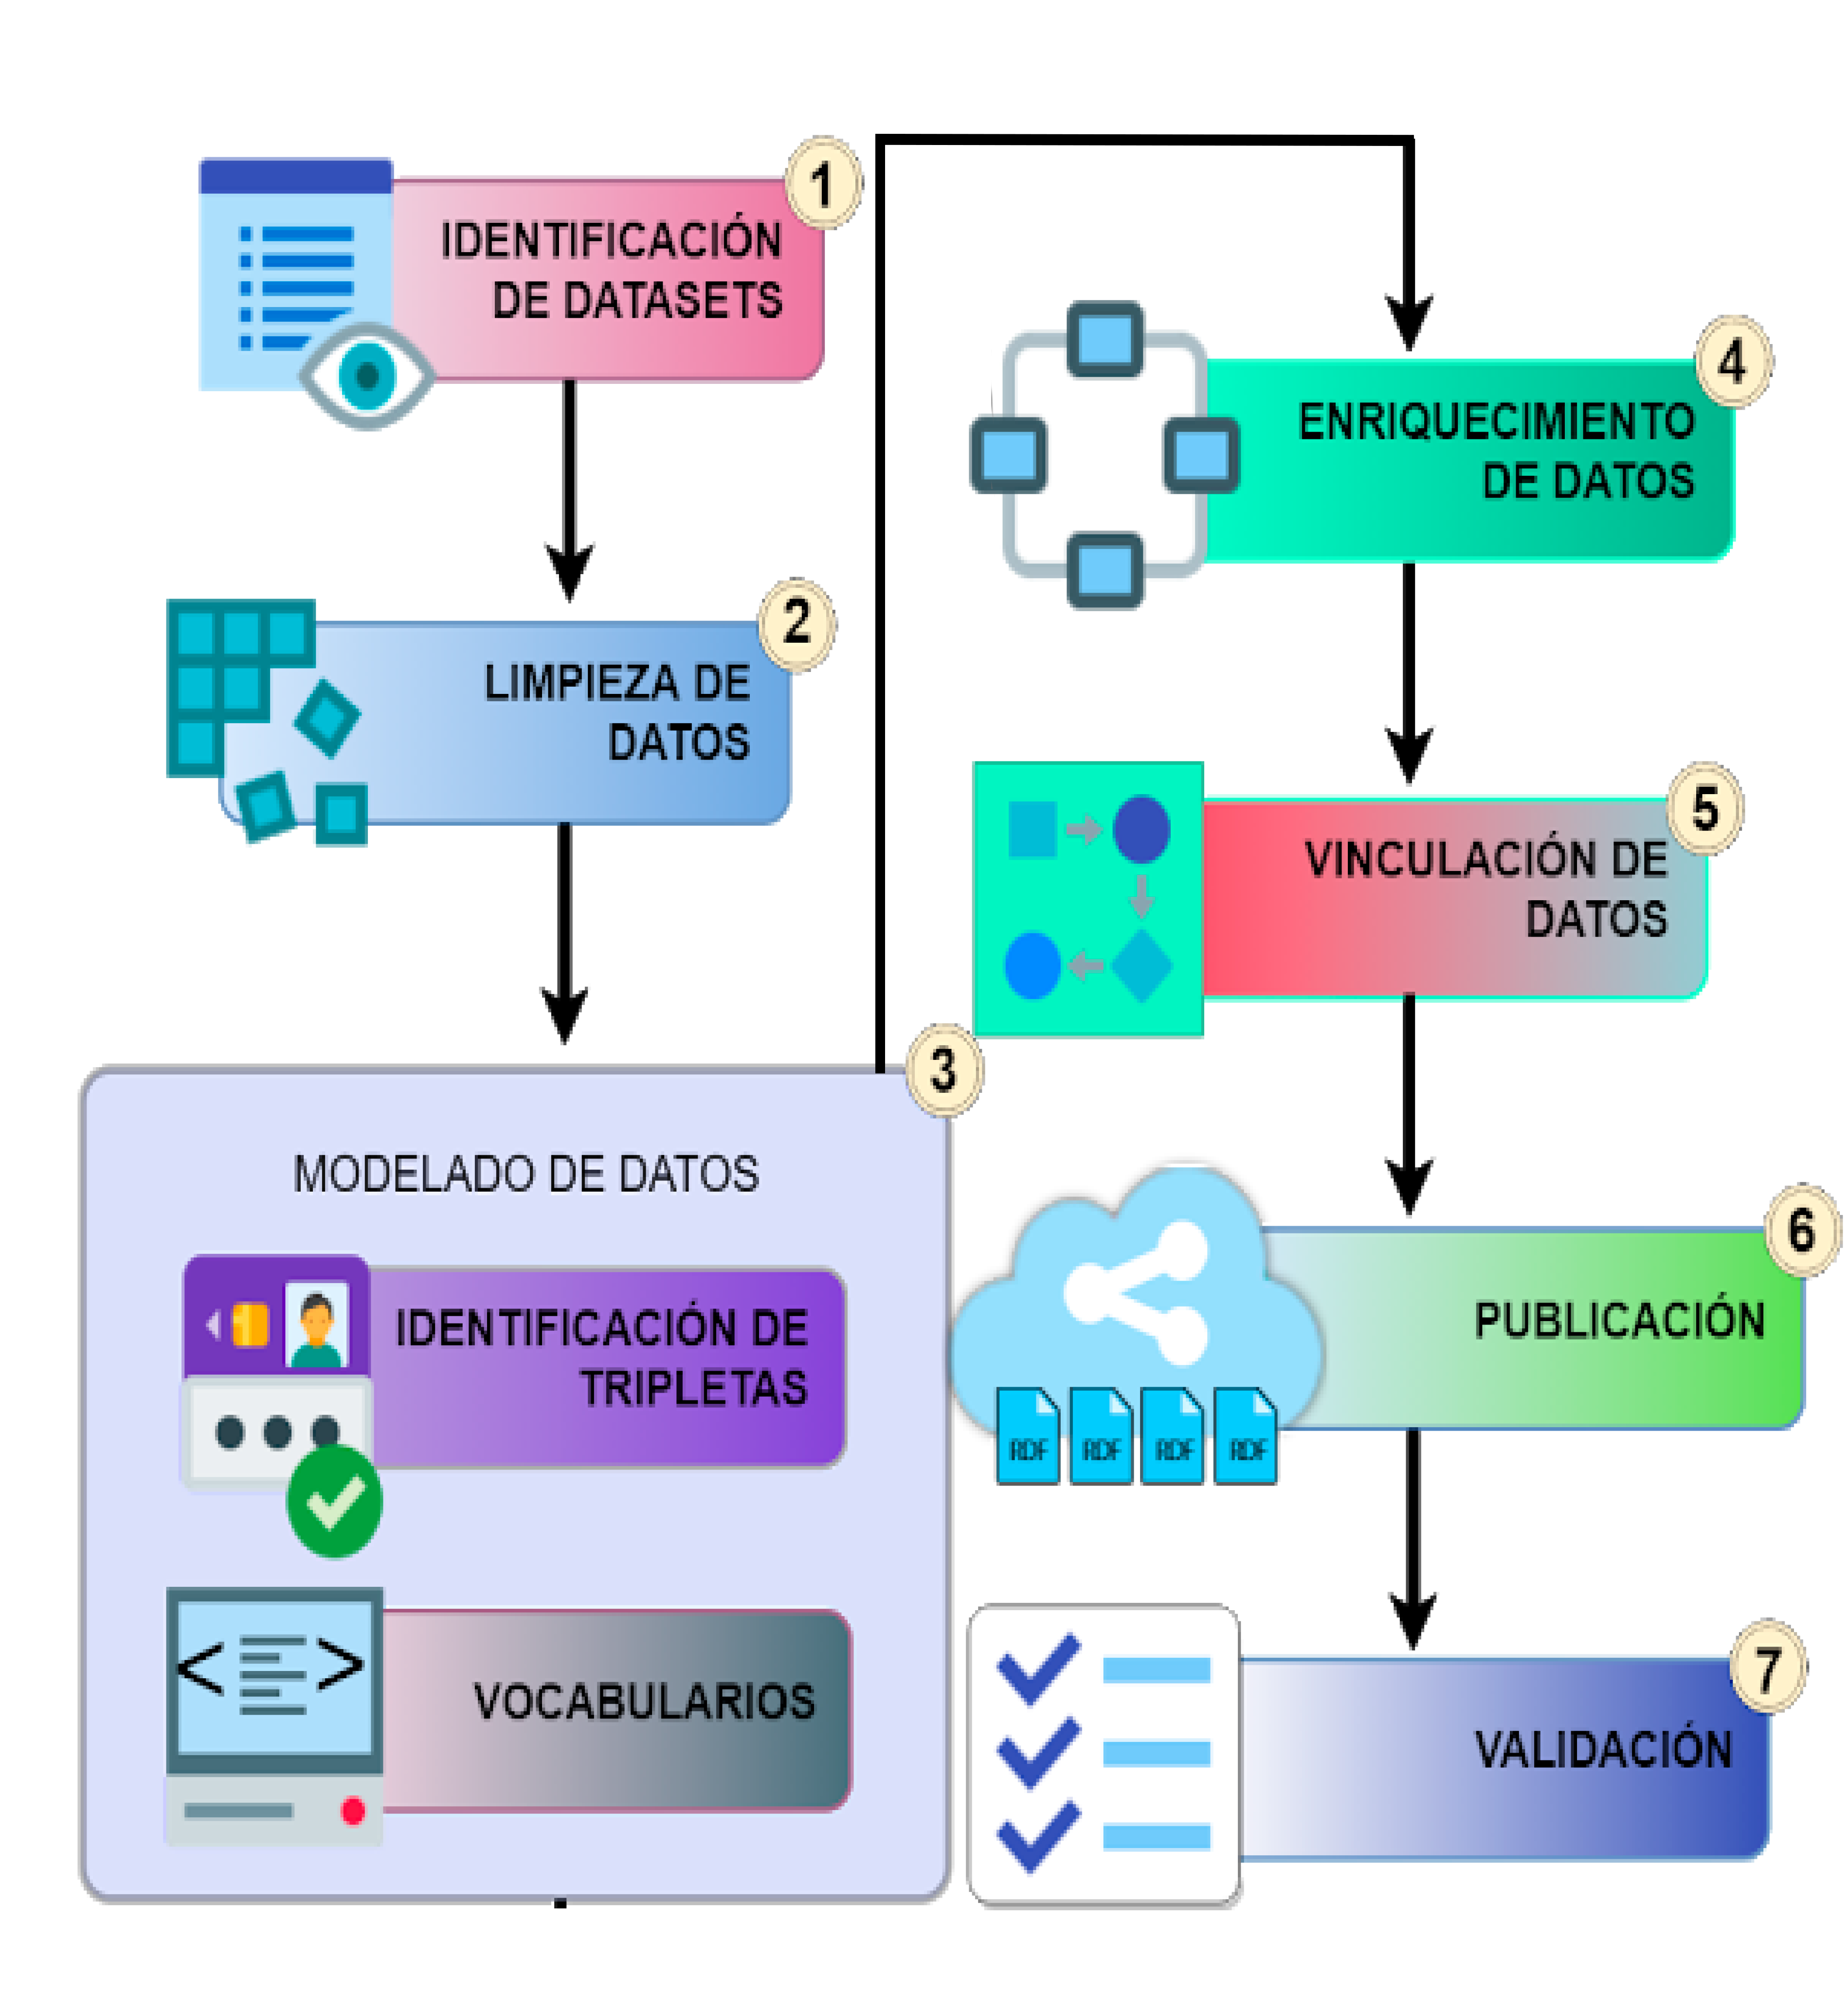
\includegraphics[scale=0.09]{../img/od-lod1.png} % Asegúrate de tener la imagen en el mismo directorio o proporciona la ruta completa
			\caption{Transformación de open data a linked open data.}
			\label{fig:od->lod}
		\end{figure}
\chapter{Beneficios de Linked Data}
Example....

\chapter{Problemas de Linked Data}
Example....

\chapter{Linked Data en bibliotecas}
Example....

\chapter{Linked Data en la actualidad}
Example....

\chapter{Conclusiones}
Example....

\begin{thebibliography}{99}
	\bibitem{1} CloudFlare. 2023.  ¿Qué es el modelo OSI?.  CloudFlare.  \url{https://www.cloudflare.com/es-es/learning/ddos/glossary/open-systems-interconnection-model-osi/}
	\bibitem{2} 12Características. 2023. HTTP (Características, concepto y funciones). 12Características. \url{https://www.12caracteristicas.com/http/}
	\bibitem{3} REDTECA. 2023. Protocolo HTTP. REDTECA. \url{https://redteca.com/hostings/http}
	\bibitem{4}OpenData Euskadi. 2023. RDF (Resource Description Framework). OpenData. \url{https://opendata.euskadi.eus/contenidos/informacion/opendata_rdf_euskadi/es_info/adjuntos/RDF.pdf}
	\bibitem{5} ARITMETICS. 2023. Qué es W3C. ARITMETICS. \url{https://www.arimetrics.com/glosario-digital/w3c}
	\bibitem{6} AWS. 2023. ¿Qué es XML?. Amazon. \url{https://aws.amazon.com/es/what-is/xml/}
	\bibitem{7}.  Eva Méndez. 2001. Resource Description Framework(RDF)	Especificación del Modelo y la Sintaxis. SIDAR. \url{http://www.sidar.org/recur/desdi/traduc/es/rdf/rdfesp.htm#basic}
	\bibitem{8} María Jesús Lamarca Lapuente. 2018. Hipertexto, el nuevo concepto de documento en la cultura de la imagen. Hipertexto. \url{http://www.hipertexto.info/documentos/rdf.htm}
	\bibitem{9} José A. Senso Ruiz. 2003. RDF: Resource Description Framework. Universidad de Granada. \url{https://arxiu-web.upf.edu/hipertextnet/numero-1/rdf.html#2.2}
	\bibitem{10} David Fernández Medina. 2003. Estudio del modelo de representación XML/RDF. Universitat Oberta de Catalunya. \url{https://openaccess.uoc.edu/bitstream/10609/1024/1/20847tfc.pdf}
	\bibitem{11} Wikipedia. 2023. Tim Berners-Lee. Wikipedia. \url{https://es.wikipedia.org/wiki/Tim_Berners-Lee}
	\bibitem{12}. Gonzalo Villareal. 2015. Linked Data, recomendaciones de la W3C. SEDICIBlog. \url{https://blog.sedici.unlp.edu.ar/2015/03/13/linked-data-recomendaciones-de-la-w3c/}
	\bibitem{13} ARITMETRICS. 2023. Qué es URI. ARITMETRICS. \url{https://www.arimetrics.com/glosario-digital/uri}
	\bibitem{14} htmlquick. 2023. URIS y URLS. htmlquick. \url{https://www.htmlquick.com/es/reference/uri-url.html}
	\bibitem{15} Fernando Tellado. 2016. ¿Se dice URL o URI?. WordPress. \url{https://ayudawp.com/se-dice-url-o-uri/}
	\bibitem{16} Microsoft. 2023. Esquemas de URI. Microsoft. \url{https://learn.microsoft.com/es-es/windows/uwp/app-resources/uri-schemes}
	\bibitem{17} MDN Web Docs. 2023. HTTP. Mozilla. \url{https://developer.mozilla.org/es/docs/Web/HTTP}
	\bibitem{18} W3C. 2015. Linked Data Platform 1.0. W3C. \url{https://www.w3.org/TR/ldp/}
	\bibitem{19} Tim Berners-Lee, Christian Bizer, Tom Heath. 2023. Linked Data - The Story So Far. tomheath. \url{http://tomheath.com/papers/bizer-heath-berners-lee-ijswis-linked-data.pdf}
	\bibitem{20} Guia de transformación de datos abierto a datos abiertos enlazados \url{https://herramientas.datos.gov.co/sites/default/files/2020-11/Guia%20Linked%20Open%20Data.pdf}
	\bibitem{21} LOD Cloud. \url{https://lod-cloud.net/}
	\bibitem{22} Linked Open Data: ¿Qué es?	\url{https://datos.bcn.cl/es/informacion/que-es}
\end{thebibliography}

\end{document}